\section{Data analysis}
\label{sec:fwkdataanalysis}

In this section, tentative procedures are outlined in order to compute and assess the eye parameters measured with the tasks described in the previous paragraph. However, due to the fact that complex algorithms and softwares need to be developed for discerning, isolating and computing specific eye parameters–as shown for example by \cite{giordano2017eyetrackersystem,jansson2013smoothpursuit,larsson2015detection}–engineering level software programming and mathematics are required. For example, the signal characteristics of fixations and smooth pursuit movements overlap to some extent, therefore the classification of fixations in the presence of smooth pursuit movements is complex \citep{larsson2015detection}. \cite{giordano2017eyetrackersystem} already implemented basic data analysis algorithms for smooth pursuit (Fourier transform of the Euclidean distance between eye gaze position and target position, i.e. positional gain) and for visually guided saccades (percentage of fixation points matching the target position), however they might not be sophisticated enough. Moreover, as \cite{smyrnis2008guidelines} discusses, there is still considerable variation of task procedures and outcome measurements in literature, which does not ease the process of finding few well-defined parameters that can be repeatedly used in genetic and clinical studies, and that there is need of standardization.

For these reasons, a further collaboration with experts in these fields is required in order to complete the framework. The results of the measurements done in the current study will stay in a raw format, waiting for further developments of the framework in the future. The diagrams automatically generated by the eye tracking software are be inspected visually and commented in \todo{Section XX. Results}.

As a general consideration about data analysis, \cite{sasson2012children} explain how children with ASD, and in particular the ones with impairments in sustaining attention, often exhibit more missing gaze data than controls, due to less focus on the stimuli or excessive blinking. It is useful then to compute results as a proportion of gaze time on screen instead of in absolute values, and control for participants who have exceeded a certain amount of missing data (a 50\% proportion of missing data should already be considered suspect), as a signal of lack of overall attention to the stimuli and to the experiment in general.


\subsection{Smooth pursuit data analysis}
\label{sec:fwksmoothpursuitanalysis}

Here it follows the discussion around the recommendations from \cite{smyrnis2008guidelines} for analyzing smooth pursuit data, in function of the framework for early ASD detection.

All pursuit performance parameters are affected by target speed. The average target speed is calculated basing on the frequency and the amplitude of target motion, therefore the amplitude of target motion needs to be reported, as well as the amplitude covered by the moving target to the right and left of the central fixation point. Pursuit performance seems to deteriorate with increasing speed.

Pursuit gain should be used as the primary outcome parameter (as also the studies reviewed in \todo{Section 2.2.1. Smooth pursuit} do) and other parameters such as frequency of catch up saccades, anticipatory saccades and square wave jerks can be used as secondary outcome. Gain needs to be defined as the ratio of eye velocity to target velocity (i.e. if pursuit performance is perfect this value should be equal to 1), and it should be preferably time weighted. The mean or the median value of pursuit gain for each target speed needs to be reported.

In a sinusoid stimulus the target velocity changes constantly, so for each segment the target velocity needs to be computed, while in triangular and trapezoidal patterns eye velocity (distance traveled divided by time) is computed for each “saccade free” segment and then divided by the constant target velocity. In order to time weight the pursuit gain, gain values at each segment are multiplied by the corresponding time and then summed. The sum of the products is then divided by the total time duration of these segments.

Since eye pursuit involves the integrated function of both the pursuit and the saccadic system, it is necessary to distinguish between smooth pursuit movements and saccades in the pursuit task records. Lower quality of pursuit could be due to two qualitatively different effects: the inability to follow the target with the same gain or the inability to suppress the saccadic system function during pursuit, resulting in intrusive saccades during pursuit.

In order to discern the records of smooth pursuit movements and saccades, it is better to use combined criteria for describing the saccades parameter thresholds (e.g. amplitude, velocity and acceleration). Once saccades onset and duration are detected they can be separated from pursuit records. Simpler criteria are not enough detailed for having a clear separation. 

\cite{smyrnis2008guidelines} strongly emphasizes that there is therefore a need for the definition of the saccade movements involved in smooth pursuit (Fig.~\ref{fig:intrusivesaccades}) and their operationalization in precise (and possibly standard) metrics:
\begin{itemize}
    \item Catch up saccades: small amplitude eye movements in the direction of target motion that bring the eye close to the target when pursuit gain is low. They serve a different purpose than intrusive saccades.
    \item Anticipatory saccades: eye movements that are in the direction of motion, take the eyes ahead of target, have amplitudes of 5 deg or more and are followed by a time interval during which the eyes virtually remain stationary.
    \item Backup saccades: eye movements performed after an anticipatory saccade, in the opposite direction, in order to bring the eyes back to the target with a saccade.
    \item Square wave jerks: pairs of small saccades 0.5–3 deg in amplitude separated by a 200–400 ms interval. Differences in definitions are found in literature about if these movements should be of opposite direction, and if they interrupt, precede or follow smooth pursuit.
\end{itemize}

Due to the different nature of these movements, computing the frequency all saccadic eye movements during pursuit as indicator of pursuit integrity means grouping together qualitatively different parameters, rendering the saccade frequency parameter not really useful. 

Differences in literature about quantitative and qualitative parameter definitions of saccadic movements in smooth pursuit highlight the need for standardization, in order to analyze and compare systematically the results of eye parameter measurements. However, this issues goes beyond the scope of this study, and it is the next step for further development of the framework and the next objective to reach in order to strengthen the reliability and the validity of all the eye tracking methodology.

\begin{figure}[h]
  \centering
  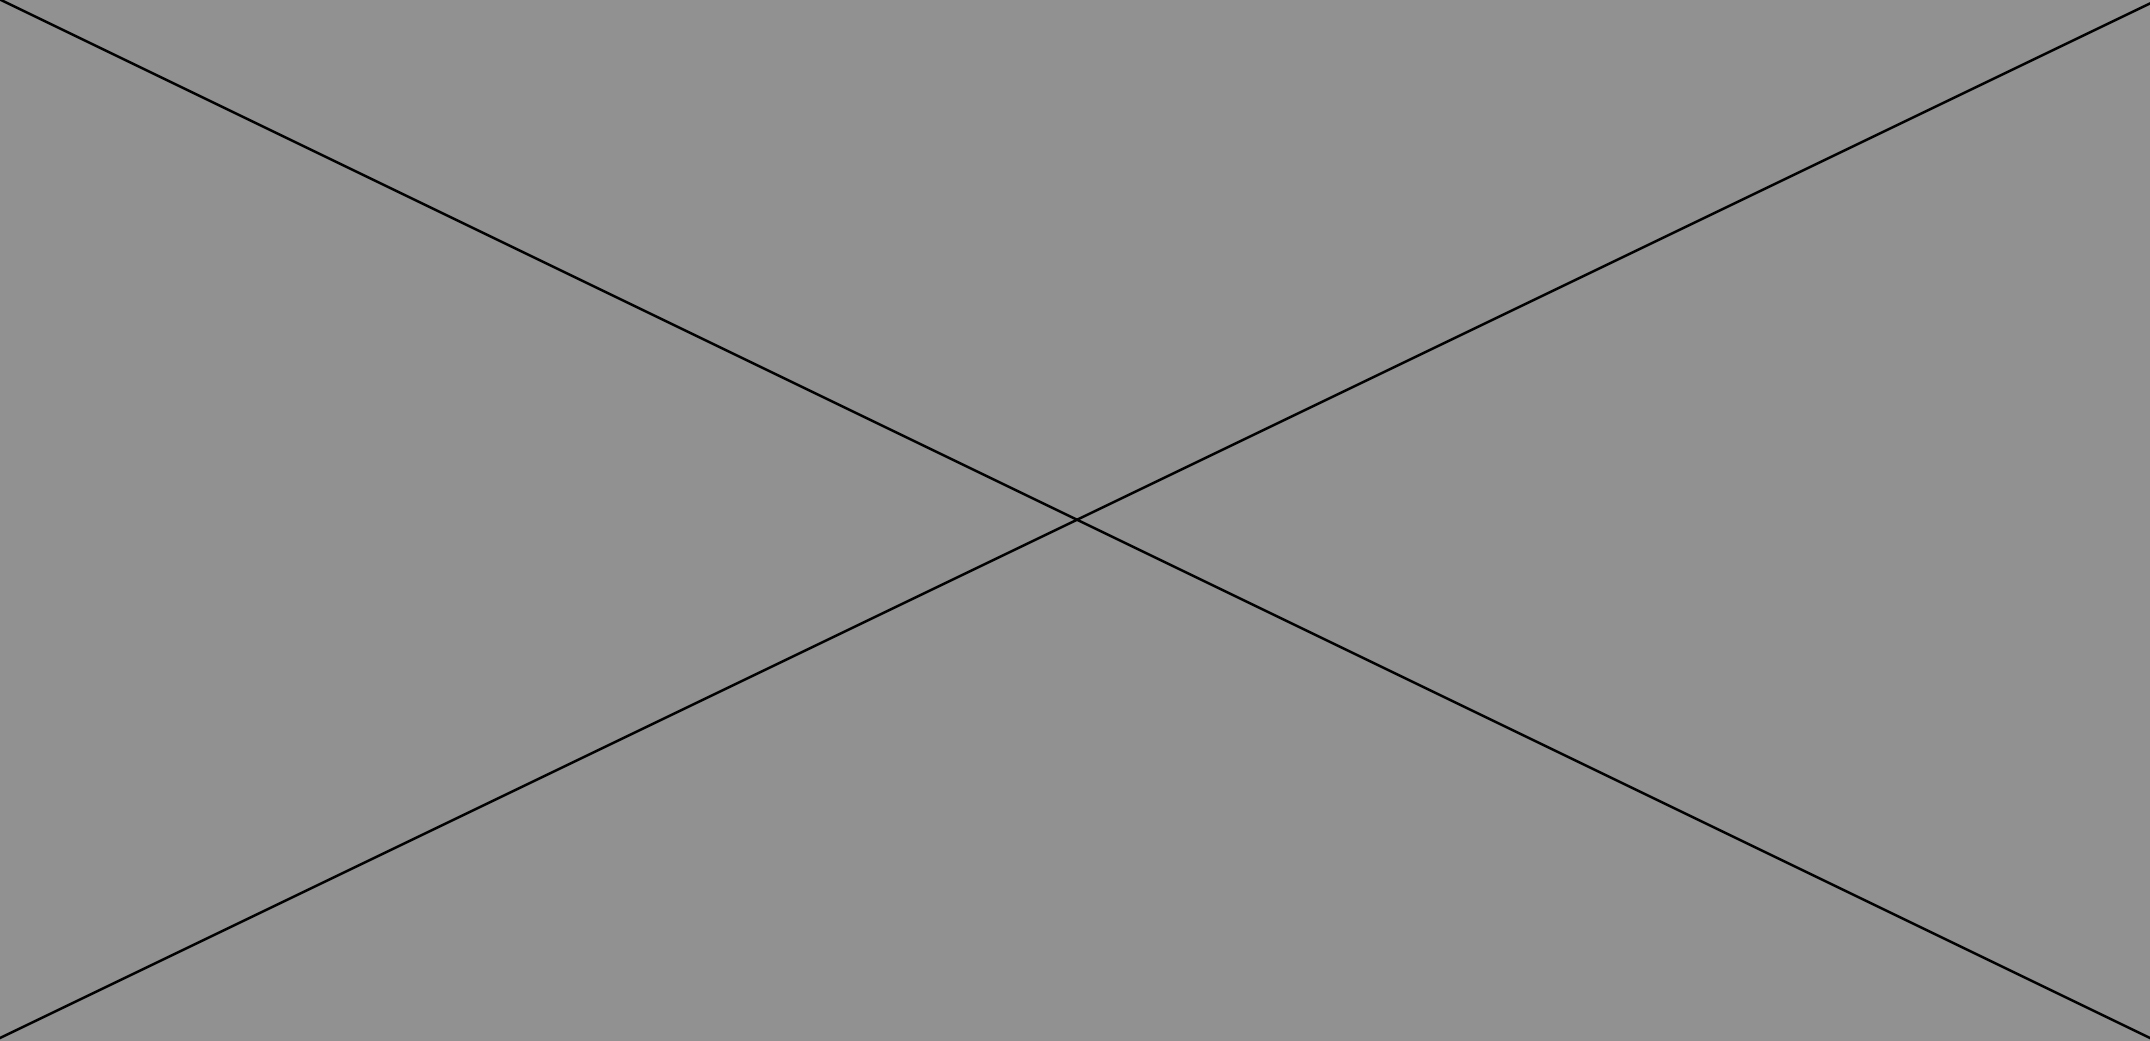
\includegraphics[width=.5\textwidth]{figures/placeholderImg.jpg}
  \caption[Saccades during smooth pursuit]{Visual example of different types of eye movements (cu = catchup saccades, sp = smooth pursuit, is = intrusive saccades, bu = backup saccades) happening during a smooth pursuit task of a trapezoidal moving stimuli. Image retrieved from \cite{randal1993smooth}.}
  \label{fig:intrusivesaccades}
\end{figure}

Discarding the pursuit data close to the direction shift points (Fig.~\ref{fig:dirchange}) allows to analyze eye movements only on a central window around the primary eye position (e.g. upward-left/right, downward-left/right), avoiding to take into account the different strategy effects in the points of a direction shift. Close to these points the pursuit of the target becomes more erratic and intrusion saccades are more frequent.

\begin{figure}[h]
  \centering
  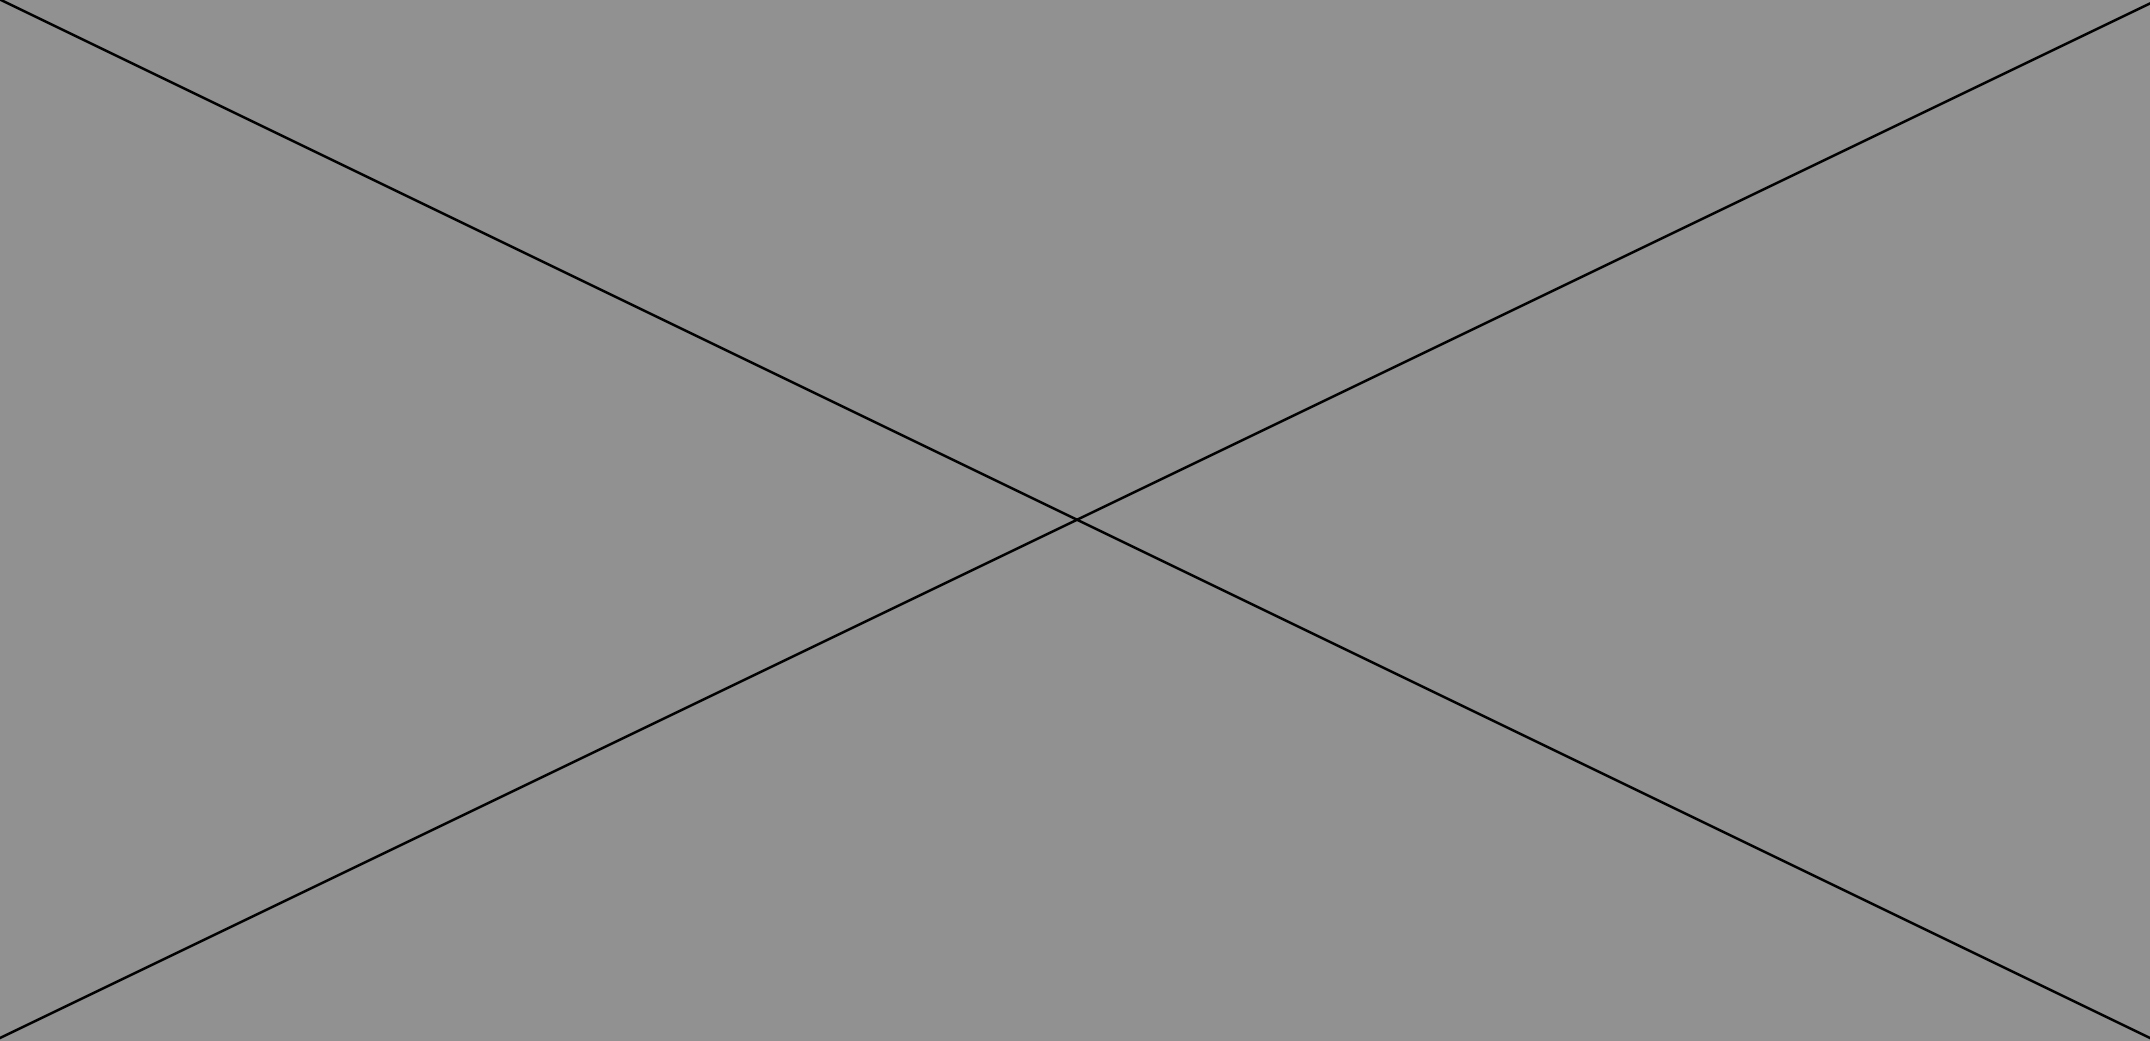
\includegraphics[width=.5\textwidth]{figures/placeholderImg.jpg}
  \caption[Discard data at turning points]{visual example of removal of the data close to direction shift points. Original picture from \cite{vonhofsten1997smoothpursuit}}
  \label{fig:dirchange}
\end{figure}

In addition to discerning smooth pursuit eye movements and saccades, artifacts (such as blinks) in the pursuit record needs to be removed (Fig.~\ref{fig:blinkartifacts}). Literature does not report a preferential way to discard artifacts, but it can be done by visual inspection or by using a pattern recognition program (using visual inspection to validate the program decisions). Probably the latter option is the more suitable for this framework, but it implies advanced computation beyond the scope of this study.

\begin{figure}[h]
  \centering
  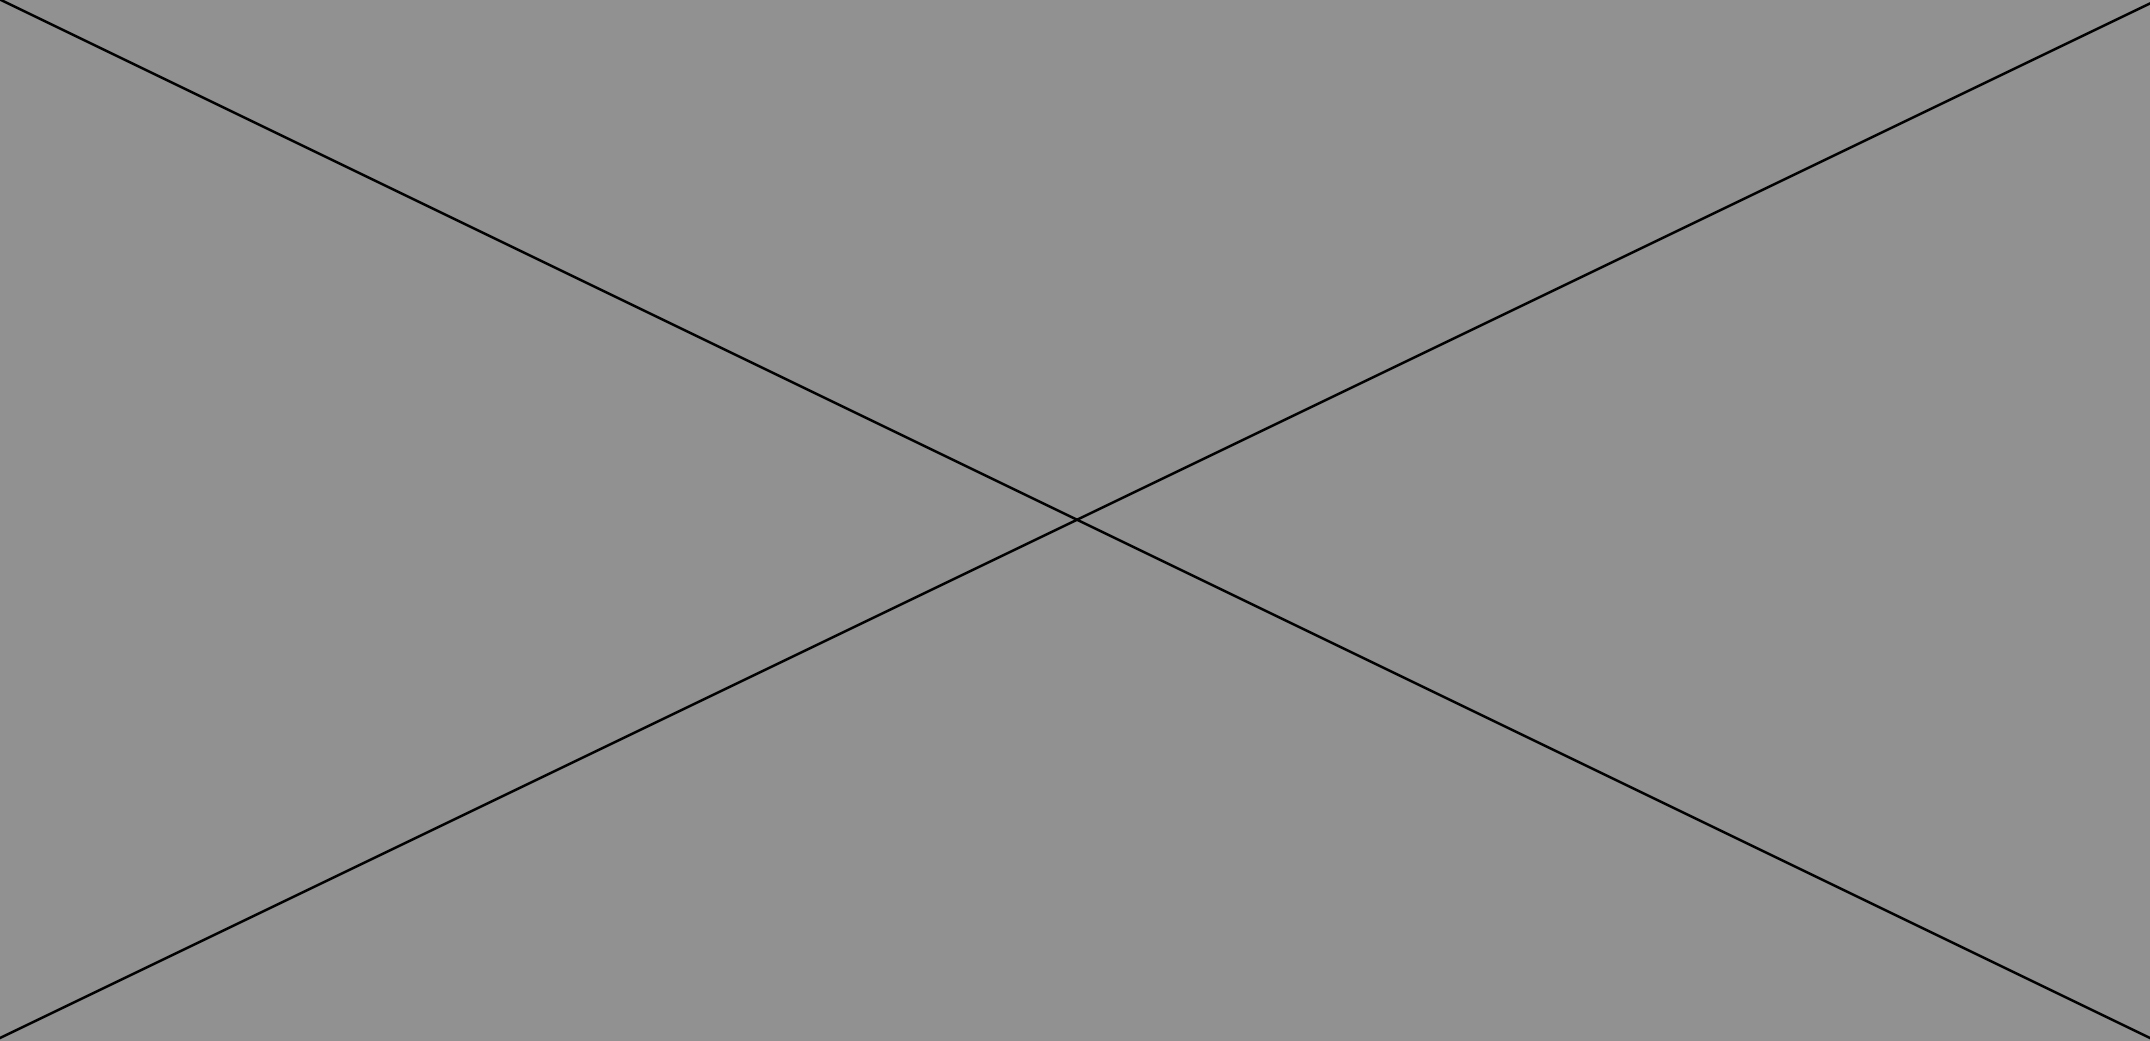
\includegraphics[width=.5\textwidth]{figures/placeholderImg.jpg}
  \caption[Blink artifact]{Example of artifact in smooth eye pursuit on trapezoidal motion stimuli. Image retrieved from \cite{randal1993smooth}}
  \label{fig:blinkartifacts}
\end{figure}

As \cite{takarae2004smoothpursuit} illustrate, in order to measure the performance in the open-loop phase of pursuit gain with a step ramp task, it is necessary to compute gain of the first catch-up saccade (defined as the ratio of eye movement amplitude to target distance) and pursuit gain during the first 100 ms after the initial saccade (defined as ratio of the average velocity of pursuit eye movement to target velocity).

For smooth pursuit tasks it is valuable to report stimulus speed (deg/s), amplitude and number of cycles.



\subsection{Saccades data analysis}
\label{sec:fwksaccadesanalysis}

\cite{johnson2016review} report that the only parameter expected to differ between ASDg and TDg is the standard deviation of saccade gain.
Here it follows the discussion around the recommendations from \cite{smyrnis2008guidelines} for analyzing saccades data, in function of the framework for early ASD detection.

Similarly to what stated in \todo{Section 3.5.1 Smooth pursuit}, combined criteria (e.g. amplitude, velocity and acceleration) needs to be used to define and describe with sufficient detail the saccades, and therefore to detect their onset and duration in the record. This level of detail allows to exclude from analysis (or analyze separately) predictive saccades (latency \(\leq\) 80 ms) and very slow onset saccades (latency \textgreater 500 or 600 ms). Rejection of artifacts can be done by visual inspection or if using a pattern recognition program (with the clinicians’ supervision).

Once the refinement process is done on the saccades records, saccade parameters prove to be easier to compute from the raw data than the smooth pursuit ones. \cite{pensiero2009saccades} show two diagrams (Fig.~\ref{fig:saccaderecordex}) which visualize examples of good and poor tracking during saccade tasks.

Since no other saccade parameter seems to help in differentiating ASDg to TDg, only the saccade gain (defined as the mean or preferably the median ratio of saccade amplitude to target amplitude) should be used as primary performance outcomes in the saccade task. With the gain mean and the number of sampled saccade records it is possible to compute the standard deviation of the gain, as index of saccade dysmetria \cite{johnson2016review}.

It is valuable to report central fixation duration (ms), peripheral target duration (ms), amplitudes of the locations for the peripheral target presentation (in degrees) and the number of trials.

\begin{figure}[h]
  \centering
  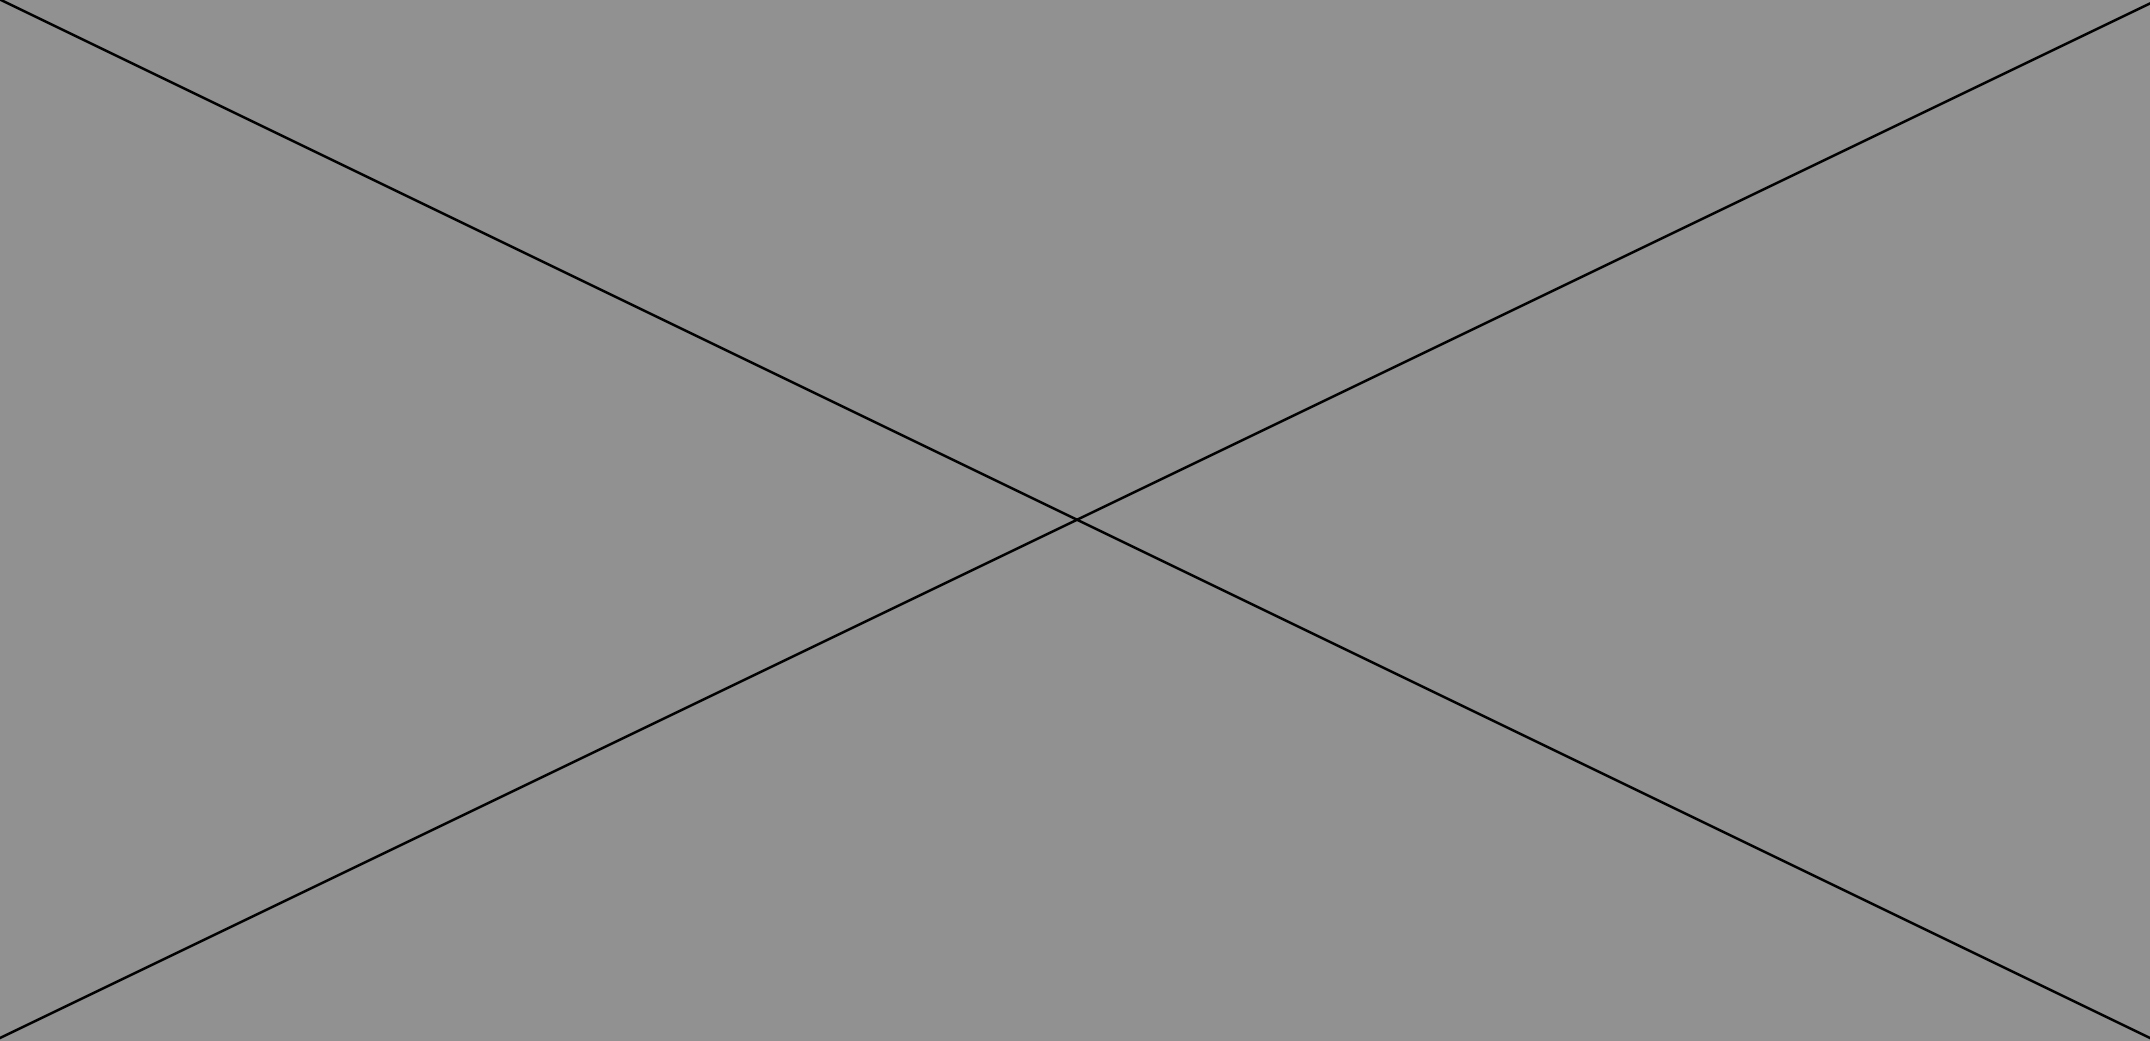
\includegraphics[width=.5\textwidth]{figures/placeholderImg.jpg}
  \caption[Saccades example graph]{Examples of good and poor tracking from \cite{pensiero2009saccades}. In the graphs are plotted the stimulus position (black), right-eye position (red) and left-eye position (blue).}
  \label{fig:saccaderecordex}
\end{figure}
